\subsection{不同的优化器原理}
可参考:\href{https://mp.weixin.qq.com/s/L9jCK5rtyq3fJZEBpLvagg}{从SGD到NadaMax,十种优化算法原理及实现}

\subsection{BGD, SGD, MBGD}
神经网络的训练过程,可以看作目标函数的优化过程,在优化过程中对模型的参数进行更新,使目标函数逐步收敛到一个最优的状态。参数优化有多种方法,目前主要是基于迭代的过程,如梯度下降、牛顿法等。其中梯度下降已经霸榜多年。目前主要有以下三种梯度下降方法:
\begin{myitemize}
	\item BGD,Batch  Gradient Descent,批量梯度下降。每次计算梯度时使用全量样本。优点:
	\begin{myitemize}
		\item 所有样本都参与了梯度的计算,异常样本带来的影响更小,训练过程更稳定
		\item 收敛速度快
	\end{myitemize}
	缺点也很明显,因为使用到了所有样本,故计算耗时更长,且要将数据全部加载,对资源要求更高,且有可能收敛到局部最优。
	
	\item SGD,Stochastic Gradient Descent,随机梯度下降。每次计算梯度时只使用一个样本,通常会对全量数据进行打乱。优点:
	\begin{myitemize}
		\item 参数更新频次高,速度快。(但从另一个角度来看,单独计算每个样本的梯度或许更耗时)
		\item 可以在线优化
		\item 每次使用一个样本的随机性可能会帮助跳出局部最优
	\end{myitemize}
	缺点:每次只是用一个样本,会放大一场样本的影响,导致训练过程不稳定。
	
	\item MBGD,Mini-Batch Gradient Descent,小批量梯度下降。每次使用一部分数据计算梯度,一次通常将全量数据划分成多个batch,与SGD类似,也会对全量数据进行打乱。优点:
	\begin{myitemize}
		\item 对比BGD,速度更快,对资源要求更低;对比SGD,振荡现象没有那么明显,比SGD会更稳定
		\item 能够一定程度避免异常样本的干扰
	\end{myitemize}
	缺点:需要考虑学习率的衰减,以及选择合适的batch size,且与BGD相比存在一定程度的振荡。
\end{myitemize}
参考资料:\href{https://lumingdong.cn/summary-of-gradient-descent-algorithm.html#%E6%A2%AF%E5%BA%A6%E4%B8%8B%E9%99%8D%E7%AE%97%E6%B3%95%E7%9A%84%E4%B8%89%E4%B8%AA%E5%8F%98%E7%A7%8D}{梯度下降算法的三个变种}。
	
\subsection{Contrastive loss, Triplet loss} 
都是一种损失函数。

Triplet loss用于训练差异较小的数据,常用于人脸识别中。以这种函数为损失函数时,输入的一个样本是一个三元组(anchor, positive, negative),anchor是随机选择的一个样本,而positive和negative分别于anchor为同类/异类数据。在学习时,Triplet loss的目的就是让anchor的表征与positive的表征尽量靠近,与negative的表征尽量疏远。那么对于一个样本来说,Triplet loss写成公式: 
$$
\mathcal{L} = max( ||f(a)-f(p)||_2^2 - ||f(a) - f(n)||_2^2 + \alpha )
$$
公式的含义也很明显,尽量使类内数据相近,类间数据相离。

Contrastive loss是对比损失,也叫zero-one损失,主要用来处理孪生网络中的paired data的关系。通常Contrastive loss的输入是两个样本,且各自都有一个标签,Contrastive loss的目标就是:如果两个样本同类,则loss更小,否则loss更大。写成公式:
$$
\mathcal{L} = d_{ij}^2 \cdot Y_{ij} + (1 - Y_{ij} )max(margin - d_{ij}, 0)^2
$$
其中,$d_{ij}$就表示样本i, j之间的距离,这个可以有多种形式的定义,$Y_{ij}$表示样本i, j的标签是否相同,margin是一个阈值,如果$d_{ij}$超过阈值则应该尽量把它们划分开。

\subsection{Normalization}
\subsubsection{Batch Normalization}
在神经网络中,前一层的输出会成为后一层的输入。当前面层的参数更新后,其输出的分布也会随之改变,经过层层的叠加,越往后的变化越大。为了拟合这些数据,深层的参数需要不断适应变化的数据,导致模型的收敛速度很慢。这里的分布指的是一层里每个神经元的分布。这种分布不一致做 \textbf{Internal Convariate Shift}(内部协变量偏移)。对于一个神经元,其取值分布会逐渐偏移,例如偏移至激活函数的饱和区,即梯度很小。

一个比较直观的方式就是对每一层的输出进行标准化。Batch Normalization 在 mini-batch 的基础上对每个神经元进行标准化,即对每个特征进行标准化。具体操作为:每一层的输入维一个 mini-batch,通过这个批次来估算每一维的均值和方差,然后对每一维进行标准化,除此之外,BN 中还对标准化后的特征进行了线性变化。
$$
\begin{array}{rlr|}
	\hline \text { Input: } & \text { Values of } x \text { over a mini-batch: } \mathcal{B}=\left\{x_{1 \ldots m}\right\} \\
	& \text { Parameters to be learned: } \gamma, \beta & \\
	\text { Output: } & \left\{y_{i}=\operatorname{BN}_{\gamma, \beta}\left(x_{i}\right)\right\} & \\
	\mu_{\mathcal{B}} & \leftarrow \frac{1}{m} \sum_{i=1}^{m} x_{i} & \multicolumn{1}{l|}{\text { // mini-batch mean }} \\
	\sigma_{\mathcal{B}}^{2} & \leftarrow \frac{1}{m} \sum_{i=1}^{m}\left(x_{i}-\mu_{\mathcal{B}}\right)^{2} & \text { // mini-batch variance } \\
	\widehat{x}_{i} & \leftarrow \frac{x_{i}-\mu_{\mathcal{B}}}{\sqrt{\sigma_{\mathcal{B}}^{2}+\epsilon}} & \text { // normalize } \\
	y_{i} & \leftarrow \gamma \widehat{x}_{i}+\beta \equiv \mathrm{BN}_{\gamma, \beta}\left(x_{i}\right) & \text { // scale and shift }
\end{array}
$$
注意上面公式中是以一个特征维度为例子,对于其他维也是一样的,其中的 $\gamma, \beta$ 都是需要学习的参数,即每个神经元会多出来两个参数来学习。上述过程是在针对训练而言的,但是在推断时该怎么办呢?对于测试数据,依然会进行标准化($\gamma, \beta$ 是在训练时学习好的,所以推断时是会被固定的),但是其均值和标准差就不是通过批次数据来计算的,而是这样:
$$
\begin{aligned}
	\mathrm{E}[x] & \leftarrow \mathrm{E}_{\mathcal{B}}\left[\mu_{\mathcal{B}}\right] \\
	\operatorname{Var}[x] & \leftarrow \frac{m}{m-1} \mathrm{E}_{\mathcal{B}}\left[\sigma_{\mathcal{B}}^{2}\right]
\end{aligned}
$$
那么测试数据的标准化就是这样的:
$$
\widehat{x}=\frac{x-\mathrm{E}[x]}{\sqrt{\operatorname{Var}[x]+\epsilon}}
$$
\textbf{为什么进行了标准化还要进行线性变换呢?}如果只是进行标准化后,其很有可能落在激活函数的线性区域,例如 sigmoid 激活函数,经过标准化后基本会落在 0 左右,而这一块区域基本是线性的,而达不到激活函数的非线性的功能,因此对齐进行了缩放和偏置,使其能够落在激活函数的非线性区域,由于 $\gamma, \beta$ 是学习得到的,因此也能满足其落在线性区的需求。这样做的一个目的就是:保障每一层的表征能力。


实际情况在进行BN时,可能是在通过激活函数之前进行 BN 或者在通过激活函数后再进行BN。\textbf{通常是在激活函数之前进行 BN},因为当输入较大时,通常激活函数的变化都较小,梯度变化不明显,故在激活函数之间就对数据进行BN,使其分布尽量稳定。

BN 的一些缺点:
\begin{itemize}
	\item 需要较大的batch以体现整体数据分布,要求 bath 的分布尽量与总体分布相近;
	\item 训练阶段需要保存每个batch的均值和方差,以求出整体均值和方差在infrence阶段使用;
	\item 不适用于可变长序列的训练,如RNN。
\end{itemize}

\subsubsection{Layer Normalization}
既然已经有了 BN,怎么还来了 LN 呢?参看 BN 的缺点,其中很重要的一点就是不适用于处理序列数据的网络,序列数据的格式通常为 $(batch\_size, seq\_len, emb\_dim)$,但是$seq\_len$ 并不都是相同的。如果对序列数据进行 BN,则需要计算每个 $time\ step$ 上每个特征的均值和方差,但是由于序列的长度是不一致的,若遇到了没有在训练集中出现过的序列长度则无法对超出的 $time\ step$ 做 BN 了。

与 BN 类似,LN 也是进行标准化后再进行线性变化。不同点在于 LN 的标准化是针对层而言的,而 BN 的标准化是针对神经元而言的。具体做法:LN 计算层中所有神经元的均值与方差,对于一个 batch 而言,则会计算出 $(batch\_size, seq\_len)$ 个均值和方差,即序列中每个元素(维度为 $emb\_dim$ 的向量)一对均值和方差,然后对同一层使用相同的均值和方差做标准化后进行线性变化即可。
$$
\mu^{l}=\frac{1}{H} \sum_{i=1}^{H} a_{i}^{l} \quad \sigma^{l}=\sqrt{\frac{1}{H} \sum_{i=1}^{H}\left(a_{i}^{l}-\mu^{l}\right)^{2}}
$$
其中 $a_i^l$ 就是第 $l$ 层的第 $i$ 个神经元。可以看到,计算的过程中不用考虑 batch 的大小,因此 batch 的大小和选择对 LN 是没有影响的。进行缩放时则与 BN 是一致的,每个神经元都有单独的缩放系数和偏置。因为不受 batch 中其他样本的影响,因此使用 LN 时不需要保存训练过程中各个 batch 的均值和方差,且训练过程和推断过程 LN 的操作是一致的。

\subsection{Dropout}

\subsection{Model Collapse}
模型坍塌,很形象啊,就是模型出现了一个漏洞,不管你输入什么东西都会漏进这个洞里。

这个主要出现在GAN的模型中。GAN通过生成器G和判别器D来使G捕捉到真实数据的分布。在训练GAN模型时会出现model collapse的现象,即G只捕捉到了真实数据的部分分布。为什么会这样呢?简单的介绍一下:当G捕捉到了真实数据的部分分布后,被D识破了,于是G就改变,从某个分布跳到了另外的分布,并且抛弃了原来的分布,于是就成了“猫鼠游戏”,D一直追着G跑,G最终并没有完全捕捉到真实数据的分布。参考:\href{https://blog.csdn.net/SPARKKKK/article/details/72598041}{GAN——ModeCollapse}。


\subsection{关于CNN的一点理解}
于DNN相比,CNN有两个特点:1)局部感知;2)权值共享。

局部感知。在CNN中每个Feature map中的一个值只于上一层的Feature map的一小部分有关。如果将CNN展开成DNN的形式,则一层中的一个神经元的输入只是上一层的某几个神经元。与全连接不同,全连接将上一层的所有信息作为输入,捕捉整体的信息。但局部感知以某个区域内的信息作为输入,捕获上一层数据中存在的局部信息 --- 特定的模式。

权值共享。CNN中的每一个filter都可以得到一个Feature map,同一个Feature map中的元素之间通过同一个filter卷积得到。或者说,同一层的神经元由一个filter产生,共享一套参数。
见Fig.\ref{fig:share_weight}。图来源于李宏毅老师的ppt。有一点需要注意,CNN模型的输入图像可能是单通道的也可能是三通道的,此时\textbf{每个filter不仅由长和宽还有深度},filter的深度与图像的通道数是相等的,所以一般来说有多少个filter就有多少个Feature map。

\begin{figure}[h]
	\centering
	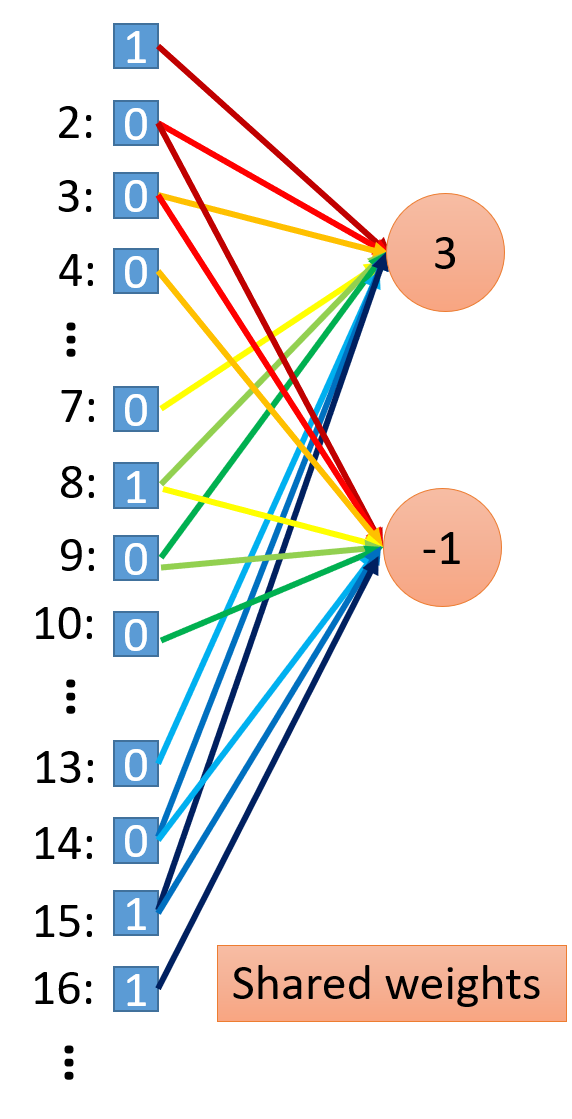
\includegraphics[width=.3\textwidth]{pics/share_weight.png}
	\caption{CNN的权值共享}
	\label{fig:share_weight}
\end{figure}

CNN的应用非常广泛,不仅是图像,在Speech、NLP等很多领域都有非常多的应用。在决定是否要使用基于CNN的模型时,需要考虑:1)数据中存在一些较小的模式,这些模式经常出现在数据中 --- 对用卷积核;2)模式与整个数据相比比较小,更大的语义信息是由很多小的模式组成的;3)进行pooling时不会破坏数据本来的含义。

在探索CNN到底学习到了什么的时候,可以在训练好模型后,通过不断优化输入的数据,来检验是什么样的输入使得基于CNN的模型中的神经元能够得到最大的激活 --- 什么样的输入使神经元最兴奋。这些主要涉及到对CNN的解释和可视化。

\subsection{深度学习中常见的参数初始化方法}
深度学习依靠大量的数据进行学习能够达到很好的效果,但是这其中依靠的是大量的参数,学习就是为这些参数找到合适的值。因此,如果一开始我们就能给这些参数设置一个比较好的值,那么学习也就省力了,这也就是如何初始化的问题了。

\subsubsection{从正态分布中采样}
或许直接将参数初始化为 0 也能进行学习,但是容易存在一些问题:学习过程缓慢,难以收敛,学习效果不好,为什么呢?如果参数全为 0,则计算的损失可能会很小,能够提供的梯度值也会很小或者根本就等于 0,这对于依靠梯度更新参数的方法来说是很致命的。因此,与全 0 相比,随机初始化反而是一个不错的选择,至少不会让梯度为 0。

\subsubsection{Glorot initialization}
但是呢,从正态分布中采样也不是一个很好的方法,为什么呢?将设我们从 $\mathcal{N}(\mu, \sigma^2)$ 中采样权重,参数的方差会影响隐层的线性变换后的方差,进而影响隐层输出的方差,这会直接影响梯度的计算,如以 sigmoid 为激活函数时,则可能落在平坦的区域 --- 也就是可能会出现梯度向后传着传着就没了或者就变得很大了。

因此一个好的初始化应该满足:各层的值(线性变换后的值、激活后的值)应该有相似的方差。为了满足前向传播时各隐层的输出值有相似的方差,以及在反向传播时,梯度也具有相似的方差,我们可以推导出参数应该又怎样的方差,这其中涉及到一些数学推导,暂时不展开。结论就是,为了前向的稳定,参数的方差应该是 $\frac{1}{f_{in}}$,为了反向传播的稳定,参数的方差应该为 $\frac{1}{f_{out}}$,其中 $\boldsymbol{W}^{fan_{in} \times fan_{out}}$。那这里有两个方差怎么办:取平均,即 $Var(\boldsymbol{W}) = \frac{1}{ \frac{fan_{in} + fan_{out}}{2}}  = \frac{2}{fan_{in} + fan_{out}}$。因此如果我们从正太分布中采样,则这个正太分布的方差应该等于 $\frac{2}{fan_{in} + fan_{out}}$,均值应该等于 0,为啥呢?在推导过程中利用了方差的一些性质,要求均值为 0。如果从均匀分布 $U(a, b)$ 中采样呢?同样需要满足 0 均值,即 $a + b = 0$,那等于多少呢?因为均匀分布的方差为 $\frac{(b - a)^2}{12}$,且 $a = -b$,因此可以解得 $b = \sqrt{\frac{6}{fan_{in} + fan_{out}}}$。

上述方法就是Xavier初始化方法(又称Glorot初始化)。当然,初始化方法还要考虑激活函数的影响,Glorot 主要用于输出均值为 0 的激活函数,如 tanh。

\subsubsection{He 初始化}
如果使用 ReLu 作为激活函数,上述的 Glorot 可能就不是那么好了,为什么呢?考虑 $ReLu(x) = max(0, x)$,将隐层的输出近一半置为 0,且 ReLu 的输出均值不为 0,不满足 Glorot 推导过程中的一些条件。为了满足各层的值方差就近似,He 初始化对权重的方差变为了 Glorot 中的两倍,为什么呢?因为 ReLu 将一般元素的值置零相当于减少了一半方差。He 初始化没有同时使用 $fan_{in}, fan_{out}$,而只使用了其中一个,实验表明这已经足够了。因此,使用 He 初始化时,正态分布的方差为 $\frac{2}{fan_{in}}$,均匀分布的的 b 为 $\sqrt{\frac{6}{fan_{in}}}$。

关于推导的一些参考:\href{https://intoli.com/blog/neural-network-initialization/}{UNDERSTANDING NEURAL NETWORK WEIGHT INITIALIZATION}、\href{https://mnsgrg.com/2017/12/21/xavier-initialization/}{Xavier Initialization}(不同激活函数下的 Glorot 初始化推导)。



\subsection{DL中的不可微操作}

\subsection{Global Max Pooling}

\subsection{Attention机制与CNN}

\subsection{权重衰减与参数正则化}

\subsection{Batch Size与Learning Rate}
模型训练过程中,\textbf{Batch Size}和\textbf{Learning Rate}是两个不可不调的参数。


\subsection{深度学习的梯度下降优化算法}


\subsection{常见损失函数及其特点}


\subsection{常见激活函数及其特点}
\subsubsection{sigmoid}
这个恐怕是无人不知无人不晓了吧,通常用于将神经元得输出转化成一个概率值:
$$
sigmoid(x) = \frac{1}{1 + e^{-x}}
$$

\subsubsection{relu}
这个算是与 sigmoid 起名的激活函数了:
$$
relu(x) = max(0, x)
$$

\subsubsection{Dice}